\chapter{Testowalność aplikacji Android}
\label{opis_problemu}

\section{Pojęcie architektury w~kontekście systemów \newline komputerowych}
\subsection{Architektura systemowa}
Systemy komputerowe są kombinacjami sprzętu komputerowego i~oprogramowania działającymi coraz częściej również w~ramach sieci komputerowej. Termin \textit{"architektura systemu"} opisuje strukturę oraz interakcję komponentów systemu komputerowego, w~tym także oprogramowania.

Systemy oprogramowania są skonstruowane tak, aby spełnić cele biznesowe organizacji. Architektura systemowa jest określana jako abstrakcyjny pomost między tymi celami. Choć droga od abstrakcyjnych celów do konkretnych systemów może być złożona, dobrą wiadomością jest to, że architektura oprogramowania może być zaprojektowana, przeanalizowana, udokumentowana i~realizowana przy użyciu znanych technik, które przyczynią się do osiągania tych celów biznesowych i~misji twórcy. 


\subsection{Architektura oprogramowania}
Istnieje wiele definicji architektury oprogramowania. Na potrzeby tej pracy autor wybrał przedstawioną w~książce Lena Bassa, Paula Clementsa i~Ricka Kazmana "Software Architecture in Practice" \cite{bib:architect:software}:

\begin{quote}
"Architektura oprogramowania jest zbiorem struktur potrzebnych do uporządkowania systemu, które zawierają elementy oprogramowania i~sprzętu oraz opisują relacje między nimi." 
\end{quote}

W systemach opartych na modelu \textit{waterfall\footnote{Iteracyjny model kaskadowy (ang. waterfall model) – jeden z~kilku rodzajów procesów tworzenia oprogramowania zdefiniowany w~inżynierii oprogramowania \cite{website:wikipedia}.}}, architektura oprogramowania tworzona jest przed rozpoczęciem pisania kodu źródłowego i~jest to bardzo poważny proces, który mógł wpłynąć na całość projektu. W~modelach projektowych opartych na metodykach zwinnych, do których autor nawiązuje i~przekonuje w~tej pracy, architektura oprogramowania może być zmieniana również podczas tworzenia systemu. Czasem jest to nawet niezbędne ze względu na dynamiczne zmiany w~wymaganiach użytkownika, lub pojawianie się kolejnych \textit{use cases}.

Analizując przytoczoną powyżej definicję architektury, można wyciągnąć następujące wnioski:

\paragraph{Architektura jest zbiorem struktur oprogramowania\newline\newline}
Struktura jest zbiorem elementów spojonych ze sobą relacjami. Systemy oprogramowania składają się z~wielu struktur, ale żadna pojedyncza struktura nie jest jeszcze architekturą. Istnieją trzy kategorie struktur architektonicznych, które odgrywają ważną rolę w~zakresie projektowania, dokumentowania i~analizy architektur:
\begin{itemize}
\item
Niektóre systemy dzielą struktury na mniejsze jednostki wykonawcze, które zwykle nazywane są modułami. Modułom przypisane są konkretne zadania obliczeniowe, które stają się podstawą przypisania pracy dla zespołów programistycznych. w~przypadku dużych projektów, elementy te (moduły) mogą być podzielone na jeszcze mniejsze części w~celu przypisania do podrzędnych zespołów. Na przykład, zaprojektowanie bazy danych dla systemu zarządzania gospodarką magazynową, produkcją, księgowością i~zasobami ludzkimi (ERP\footnote{ERP - Enterprise Resource Planning (ang.) – planowanie zasobów przedsiębiorstwa}) w~dużym przedsiębiorstwie może być zbyt skomplikowane dla jednego zespołu i~realizacja tego celu musi zostać podzielona na wiele części. Moduł logistyczny może stać się jednym modułem, moduł produkcyjny drugim, a~moduł wspomagania księgowości - trzecim. Również inne funkcjonalności systemu muszą czasem zostać podzielone i~przypisane do osobnych zespołów wdrożeniowych;
\item
Inne struktury systemowe mogą być dynamiczne, co oznacza, że dotyczą sposobu, w~jaki poszczególne elementy współdziałają ze sobą w~czasie wykonywania planowanych funkcji systemu. Jeżeli system ma być zbudowany jako zestaw usług, to usługi te współdziałają z~infrastrukturą i~wymagają synchronizacji; 

\item
Trzeci rodzaj struktury opisuje odwzorowanie elementów programowych na elementy systemowe: organizacyjne, instalacyjne, uruchomieniowe i~rozwojowe. Na przykład, moduły mogą być przypisane do zaprogramowania przez zespoły oraz przypisane do odpowiednich miejsc w~strukturach systemu, tak aby później nie było problemów chociażby z~ich testowaniem.
Te odwzorowania nazywane są \textit{alokacyjnymi}.

\end{itemize}

\paragraph{Architektura jest pojęciem abstrakcyjnym\newline\newline}
Ponieważ architektura zawiera struktury, a~struktury te zawierają elementy i~relacje między nimi, wynika z~tego, że architektura łączy te elementy systemowe ze sobą wykorzystując relacje. Oznacza to, że architektura pomija pewne informacje, które nie są użyteczne z~punktu widzenia systemu, a~w szczególności takie, które nie są ze sobą powiązane żadną relacją. Zatem architektura jest przede wszystkim abstrakcją systemu, który wybiera pewne szczegóły i~ukrywa inne. We wszystkich nowoczesnych systemach elementy współdziałają ze sobą za pomocą interfejsów, które dzielą dany element na części publiczne i~prywatne (wewnętrzne). Architektura zajmuje się stroną publiczną tego podziału, a~prywatne interakcje między funkcjami, czy nawet funkcje pełniące tylko zadania pomocnicze, nie są elementem architektonicznym. Taki rodzaj abstrakcji jest niezbędny do opisania systemu w~możliwie najprostszy i~zrozumiały sposób.

\paragraph{Każdy system komputerowy posiada architekturę oprogramowania\newline\newline}
Każdy system można pokazać w~sposób opisany w~poprzednich paragrafach, czyli jako zestaw elementów i~relacji między nimi. W~najprostszym przypadku - cały system będzie pojedynczym elementem, ale architektura opisana w~ten sposób będzie bezużyteczna.

Nawet jeżeli każdy system posiada architekturę, to nie znaczy, że architektura ta jest znana. Zdarza się, że ludzie, którzy ją tworzyli, już nie pracują w~danym przedsiębiorstwie, a~dokumentacja zaginęła lub, co gorsze, w~ogóle nie była tworzona. Jeśli do tego kod źródłowy nie został zachowany, zostaje tylko binarny kod wykonywalny, który niekoniecznie może być pomocny przy analizie systemu.
Różnica pomiędzy architekturą systemu a~jej reprezentacją polega na tym, że architektura może istnieć niezależnie od specyfikacji systemu.  Warunkiem koniecznym do odtworzenia systemu jest jej zapisana dokumentacja.

\paragraph{Architektura obejmuje również zachowanie systemu\newline\newline}
Zachowanie się każdego elementu architektury może być również jej częścią, o~ile czynność ta wnosi jakieś nowe informacje i~wpływa pozytywnie na zrozumienie systemu. Reprezentowanie, jak elementy współdziałają ze sobą, jest częścią definicji architektury, opisanej w~poprzednich paragrafach. Schematy blokowe, które często przedstawiane są jako architektura systemu, w~gruncie rzeczy nią nie są. Patrząc na nazwy pól (bazy danych, graficzny interfejs użytkownika, etc.), można sobie wyobrazić funkcjonalność i~zachowanie odpowiednich elementów, ale wypływają one w~większości z~wyobraźni obserwatora i~nie opierają się na żadnej udokumentowanej informacji. To nie znaczy, że dokładne zachowanie i~wydajność każdego elementu muszą być udokumentowane w~każdym przypadku - niektóre zachowania systemu nie leżą w~grupie zainteresowań architekta. Jednak jeżeli interakcja pomiędzy poszczególnymi elementami jest kluczowa dla działania systemu - powinna ona zostać udokumentowana.

\paragraph{Nie wszystkie rodzaje architektur są odpowiednie\newline\newline}
Definicja architektury nie specyfikuje niestety, która architektura jest dla danego systemu odpowiednia bądź nie - lub - mówiąc bardziej dosadnie, która jest dobra, a~która zła. Jak autor wykaże w~kolejnych rozdziałach, również w~przypadku systemu Android wybór odpowiedniej architektury jest kluczowy dla testowalności i~pielęgnowalności  oprogramowania tworzonego dla tej platformy.

\section{Architektura Android}
Architektura Android przez wielu opisywana jest jako \textit{Java on Linux}, czyli programowanie w~Javie pod Linuksem. Jednakże jest to stwierdzenie zbyt ogólne, biorąc pod uwagę złożoność całej platformy. Całość systemu zawiera bowiem w~sobie komponenty, które układają się w~pięć głównych warstw: \textit{Android applications}, \textit{Android Framework}, \textit{Dalvik virtual machine}, \textit{user-space native code} oraz \textit{Linux kernel} \cite{bib:hacker:handbook} (rysunek \ref{fig:ch3_android_architecture_1}).

\begin{figure}[!htb]
    \centering
    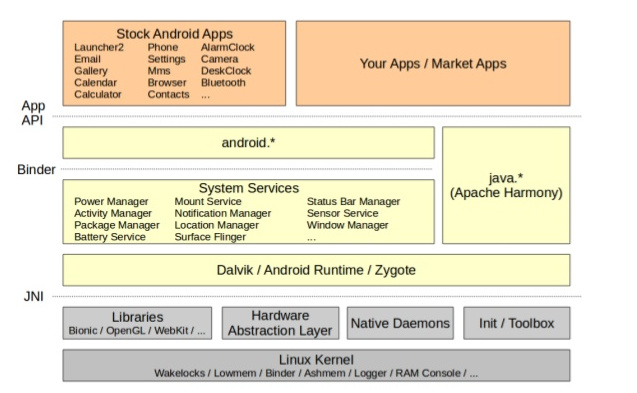
\includegraphics[width=13cm]{imgs/ch3_android_architecture_1.jpg}
    \caption
{Przegląd architektury Android \cite{website:android:przegladarchitektury}.}
    \label{fig:ch3_android_architecture_1}
\end{figure} 

Aplikacje Android pozwalają programistom rozszerzać i~ulepszać funkcjonalność urządzeń, bez konieczności sięgania do niższych warstw systemu. W~zamian framework Androida dostarcza developerom bogate środowisko użytkownika, które pozwala na dostęp do różnych udogodnień, jakie urządzenie z~tym systemem jest w~stanie programiście zaoferować. Jest to swoiste połączenie pomiędzy aplikacjami a~wirtualną maszyną Dalvika, które zezwala na konfigurowanie interfejsu użytkownika (UI\footnote{User Interface}), dostęp do baz danych oraz przekazywanie informacji pomiędzy poszczególnymi komponentami aplikacji.

Zarówno aplikacje jak i~opisywany \textit{framework} napisane są w~języku Java i~wykonywane na wirtualnej maszynie Dalvika (\textit{DalvikVM}). Jest to specjalnie zaprojektowana wirtualna maszyna z~własnym kodem bajtowym, zoptymalizowana pod jądro Linuxa i~pozwalająca na uruchamianie aplikacji androidowych. Niestety, nie wszystkie biblioteki wykorzystane przy jej tworzeniu udostępnione są na zasadzie wolnych licencji.

Natywne elementy kodu Androida zawierają usługi systemowe, usługi sieciowe oraz różnego rodzaju biblioteki, między innymi \textit{WebKit} i~\textit{OpenSSL}. 

Najniższą warstwą, a~zarazem podstawą systemu Android jest jądro Linuxa. Android dokonał licznych uzupełnień i~zmian w~jego źródłach, z~których niektóre mają swoje negatywne konsekwencje dla bezpieczeństwa. Przykładem jest luka \textit{Stagefright}, pozwalająca uzyskać dostęp do pamięci i urządzeń peryferyjnych smartfona przy pomocy specjalnie spreparowanej wiadomości MMS \cite{website:android:bezpieczenstwo}. Sterowniki znajdujące się w~jądrze systemu zapewniają również dodatkowe funkcje, takie jak dostęp do kamery, sieci Wi-Fi oraz dostęp do innych urządzeń sieciowych. Szczególnie godny uwagi jest sterownik \textit{Binder}, który realizuje komunikację między procesami \cite{bib:hacker:handbook} (IPC\footnote{Inter-Process Communication}).

\section{Obszary testowe}
\label{obszary_testowe}
Z punktu widzenia projektu, idealnie byłoby mieć możliwość przetestowania każdej linii kodu. Autor zdaje sobie sprawę, że w~wielu przypadkach jest to niemożliwe, a~nawet bezcelowe, więc dopuszcza się możliwość ograniczenia testowania do kluczowych elementów kodu źródłowego i~kluczowych funkcjonalności. Na przykład zwykle nie jest potrzebne testowanie \textit{setterów}, \textit{getterów}\footnote{\textit{Settery} i~\textit{gettery} - w~programowaniu metody służące do kontrolowania zmian wartości zmiennych}, czy funkcji należących do standardowych bibliotek, gdyż zapewne zostały przetestowane już podczas procesu ich tworzenia. 

Według \cite{bib:android:testing:learning}, można wyróżnić trzy główne obszary testowania:

\begin{itemize}
\item{Cykle życia aktywności;}

Należy przetestować, czy aktywność przechodzi prawidłowo przez swoje cykle życia. Trzy główne pętle do przetestowania znajdują się na rysunku \ref{fig:sample_figure}.
\begin{figure}[!htb]
    \centering
    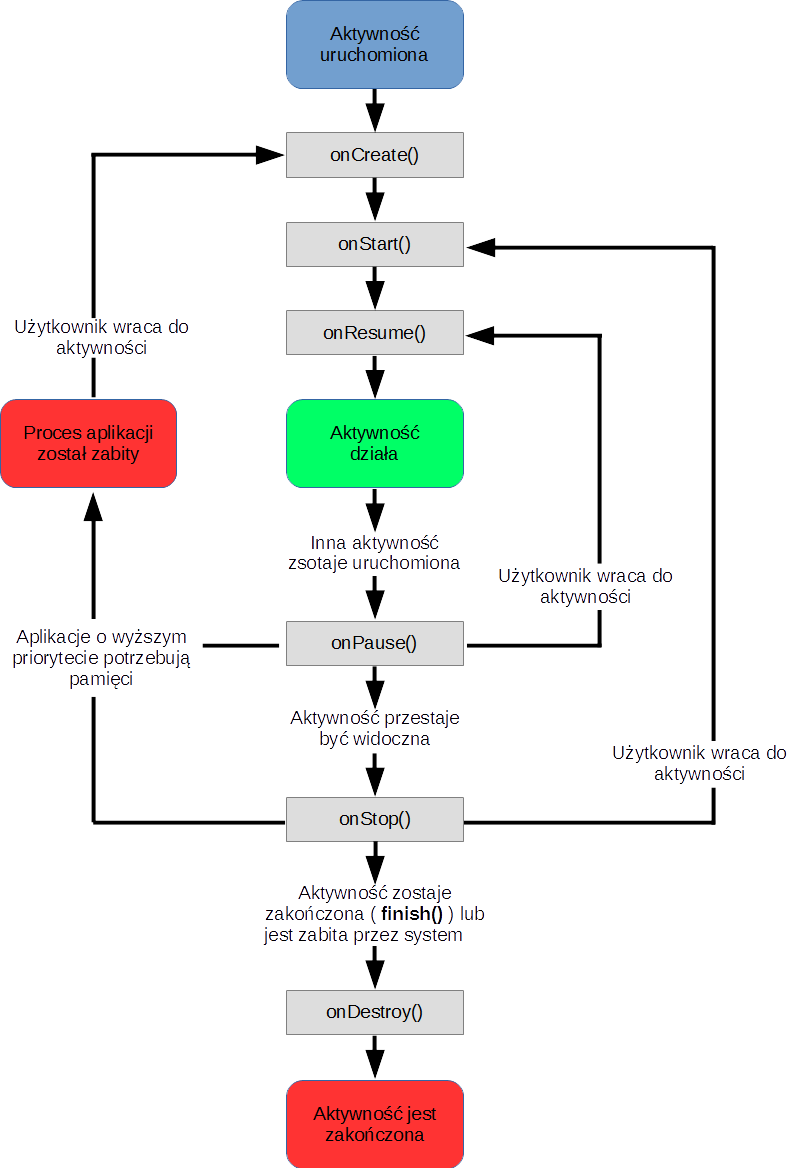
\includegraphics[width=10cm]{imgs/ch2_activity_lifecycle.png}
    \caption{Cykl życia \textit{Activity} \cite{website:android:aktywnosci}}
    \label{fig:sample_figure}
\end{figure} 

\item{Dostęp do baz danych i~do systemu plików;}

Należy sprawdzić, czy operacje dostępowe przeprowadzane są poprawnie, a~jeżeli nie, to czy również poprawnie działa obsługa błędów. Można to testować na dwa sposoby: albo na niskim poziomie, izolując warstwę użytkownika, albo bezpośrednio z~aplikacji. Do testowania na niskim poziomie można wykorzystywać dostarczane przez framework Androida w~pakiecie \texttt{android.test.mock} \textit{zaślepki}\footnote{Zaślepka (stub) - szkieletowa albo specjalna implementacja modułu używana podczas produkcji lub testów innego modułu, który tę zaślepkę wywołuje albo jest w~inny sposób od niej zależny. Zaślepka zastępuje wywoływany moduł. [wg. IEEE 610]}

Według dokumentacji Android \cite{website:android:manual} możliwe są następujące opcje przechowywania danych:

- \textit{Shared Preferences}, czyli zachowywanie podstawowych danych w~parach klucz - wartość;

- pamięć wewnętrzna urządzenia - do zachowywania danych niepublicznych;

- zewnętrzna karta pamięci - do zachowywania danych publicznych;

- baza danych SQLite - do przechowywania danych w~prywatnej bazie danych;

- zasoby sieciowe - jako baza danych współdzielona pomiędzy urządzeniami.

Wszystkie te opcje korzystają ze wspólnego zestawu funkcji\footnote{Na przykład do obsługi plików używa się \textit{getFileDir(), getDir(), deleteFile()} itp.}, które tester powinien wziąć pod uwagę przy tworzeniu przypadków testowych.

\item{Fizyczną charakterystykę urządzenia;}

Android został zaprojektowany do pracy na wielu różnych typach urządzeń, od telefonów do tabletów i~telewizorów. Programiści muszą tolerować pewną zmienność zachowań projektowanych funkcji i~zapewnić elastyczny interfejs użytkownika, który dostosowuje się do różnych konfiguracji ekranu czy sieci.

Należy sprawdzić, czy aplikacja działa poprawnie na wszystkich urządzeniach, na których można ją uruchomić. To, że działa świetnie na smartfonie, nie znaczy że działa poprawnie na tablecie, a~to że działa na tablecie jednej firmy nie wyklucza awarii na tym samym urządzeniu wyprodukowanym przez innego producenta. Elementy, które należy testować w~tym zakresie, to:

- możliwości sieciowe;

- rozdzielczość ekranu;

- gęstość ekranu;

- rozmiar ekranu;

- czułość sensorów;

- klawiaturę i~inne urządzenia wejściowe;

- lokalizację GPS;

- zewnętrzne karty pamięci.

Android framework pewne parametry dostosowuje automatycznie, ale nie zwalnia to projektantów przed wykonaniem zestawu niezbędnych testów również w~tym obszarze.

\end{itemize}

\section{Standardowe podejście przy tworzeniu aplikacji}
\label{standardowe_podejscie}
W większości przypadków aplikacje z~przeznaczeniem dla systemu Android pisane są według schematu widocznego na rysunku \ref{fig:opis_problemu}:

\begin{figure}[!htb]
    \centering
    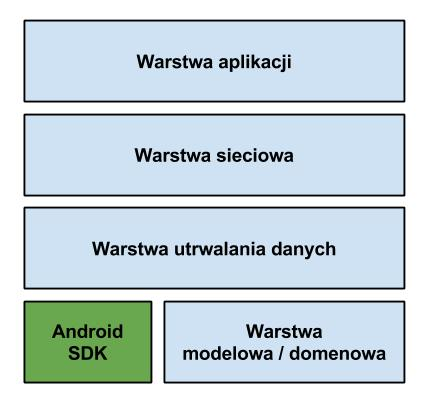
\includegraphics[width=7cm]{imgs/ch3_opis_problemu_1.jpg}
    \caption
{Podejście „standardowe” przy tworzeniu aplikacji dla systemu Android.}
    \label{fig:opis_problemu}
\end{figure} 

\newpage
Najniższa warstwa to Android SDK. Każda z~kolejnych warstw oprogramowania korzysta z~warstwy poniżej, a~co za tym idzie, dziedziczy również zależności z~warstwy Android SDK. Analizując taką strukturę aplikacji dostępnych pod Androidem można zaobserwować, że w~wielu z~nich:
\begin{itemize}
\item
nie jest zachowana zasada pojedynczej odpowiedzialności;
\item
warstwa odpowiedzialna za logikę domenową jest pomieszana z~warstwą UI (User Interface);
\item
logika UI jest pomieszana z~asynchronicznym pobieraniem danych;
\item
funkcje \textit{callback\footnote{Wywołanie zwrotne (ang. callback) jest to technika programowania będąca odwrotnością wywołania funkcji. Zwykle korzystanie z~właściwości konkretnej biblioteki polega na wywołaniu funkcji (podprogramów) dostarczanych przez tę bibliotekę. w~tym przypadku jest odwrotnie: użytkownik jedynie rejestruje funkcję do późniejszego wywołania, natomiast funkcje biblioteki wywołają ją w~stosownym dla siebie czasie  \cite{website:wikipedia}.}} można znaleźć w~całym kodzie;
\item
elementy warstwy UI: Activity i~Fragmenty potrafią mieć tysiące linii kodu;
\item
w większości plików aplikacji na każdej warstwie istnieją odwołania do środowiska Android;
\item
istnieją problemy z~wprowadzeniem testów jednostkowych.
\end{itemize}

Spowodowane jest to dwoma czynnikami: pierwszy to trudność w~wyodrębnieniu obszarów testowych wymienionych w~części \ref{obszary_testowe} z~powodu zbyt dużego sprzężenia między warstwami (\textit{couplingu}), a~drugi – pracochłonność w~pisaniu testów. Jeżeli granica pomiędzy kolejnymi warstwami oprogramowania nie jest jasno wyznaczona, liczba testów do zaprojektowania rośnie znacząco.


\section{Trudności w~testowaniu aktualnej struktury \newline aplikacji}
\label{testowanie_starej_struktury}

Weźmy dwie funkcjonalności przedstawione na rysunku \ref{fig:testowanie_klas}: funkcjonalność \textbf{A} opisaną za pomocą kodu z~jedną instrukcją warunkową \textit{„if”}, oraz funkcjonalność \textbf{B}, w~której mamy dwie zależne od siebie instrukcje \textit{„if”}, czyli cztery możliwe decyzje programowe. 

\begin{figure}[!htb]
    \centering
    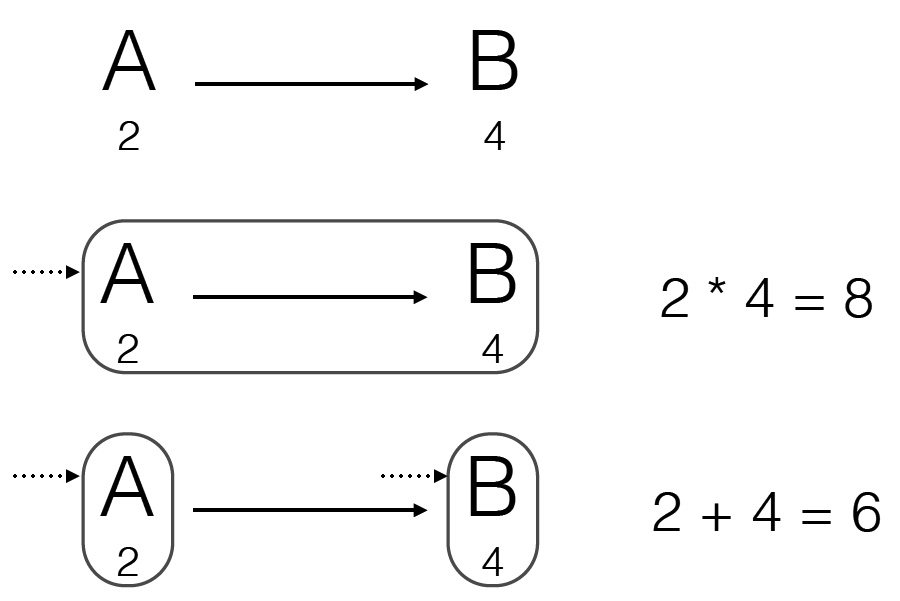
\includegraphics[width=8cm]{imgs/ch3_przyklad_testowania_klas_pl.png}
    \caption
{Różnice w~testowaniu klas osobno i~razem. \textit{"Integrated Tests are a~Scam"} - schemat autorstwa J.B. Rainsbergera  \cite{website:android:testowanieklas}.}
    \label{fig:testowanie_klas}
\end{figure} 
\newpage
Testując te funkcjonalności razem (z powodu sprzężenia nie ma innego wyjścia) należy wykonać łącznie 8 testów, co zostało przedstawione na równaniu \ref{eq:test1}:
\begin{equation}
2*4=8 \label{eq:test1}
\end{equation}

Testy te równocześnie przestają być testami jednostkowymi, gdyż łączą w~sobie kilka funkcjonalności i~stają się przez to testami integracyjnymi. Testując natomiast te funkcjonalności osobno, trzeba wykonać łącznie 6 testów jednostkowych (równanie \ref{eq:test2}):
\begin{equation}
2+4=6 \label{eq:test2}
\end{equation}
W~powyższym przykładzie oczywiście nie widać zbyt wielkiej optymalizacji, ale w~aplikacjach z~kodem, który dostarcza setki czy tysiące decyzji, różnica będzie znacząca.

Również w~przypadku architektury aplikacji Android, jeżeli zachodzi konieczność testowania każdej klasy lub pojedynczej funkcji w~powiązaniu z~\textit{Android SDK}, liczba testów jednostkowych zauważalnie wzrośnie.

\section{Pielęgnowalność aplikacji Android}
\label{pielegnowalnosc_aplikacji}
W realnym świecie niestety bardzo rzadko istnieje możliwość tworzenia aplikacji od początku. W~większości przypadków programiści muszą borykać się z~kodem, który ktoś już kiedyś napisał, a~dotyczy to w~zasadzie wszystkich większych projektów informatycznych. Przeanalizujmy jako przykład  aplikację \textit{Gmail}, największy program pocztowy wydawany przez firmę Google\footnote{Gmail – bezpłatny serwis webmail posługujący się technologią AJAX, stworzony i~rozwijany przez przedsiębiorstwo Google. W~lutym 2016 roku liczba jego użytkowników przekroczyła miliard \cite{website:wikipedia}.}. Wychodzą ciągle nowe wersje, ale trudno wyobrazić sobie sytuację, że któraś z~nich została po prostu napisana od nowa. W~takich przypadkach mamy do czynienia z~tzw. \textit{kodem zastanym}.

O ile kod pisany był w~sposób przejrzysty, dobrzy programiści są w~stanie dobudować nowe części aplikacji, nawet nie mając dokumentacji do starszej części. Wiele firm programistycznych stosuje podejście, że sam kod programu jest zarówno jego dokumentacją. Rozsądne nadawanie nazw zmiennym oraz umieszczanie rzeczowych komentarzy pozwala programistom zrozumieć swoich poprzedników, a~automatycznym narzędziom, takim jak \textit{JavaDoc\footnote{Javadoc – narzędzie automatycznie generujące dokumentację na podstawie zamieszczonych w~kodzie źródłowym znaczników w~komentarzach. Javadoc został stworzony specjalnie na potrzeby języka programowania Java przez firmę Sun Microsystems \cite{website:wikipedia}.}} lub \textit{Doxygen\footnote{Doxygen – generator dokumentacji dla języków C++, C, Java, Objective-C, Python, IDL, Fortran i do pewnego stopnia dla PHP, C\#, D oraz ActionScript. Obsługuje następujące formaty wyjściowe: HTML, CHM, RTF, PDF, LaTeX, PostScript oraz strony man \cite{website:wikipedia}.}} wygenerować całkiem wyczerpującą dokumentację.

Gorsza sytuacja jest z~testowaniem. Jeżeli produkt nie był tworzony dotychczas z~zastosowaniem techniki TDD, praca jaką należałoby wykonać przy pisaniu unit testów do gotowego kodu może być ogromna. Ponadto istnieje ryzyko, że tester chcąc sprostać wymaganiom osób zarządzających projektem będzie tak pisał testy jednostkowe, aby pokrywały jak największą część kodu, niekoniecznie przy tym wnosząc jakąś wartość w~sprawdzenie niezawodności aplikacji.

%Jedno z~możliwych rozwiązań zaproponowane zostało w~rozdziale \ref{legacy_code}